\section{Anomaly Detection and Cancellation}

\subsection{Definition of Anomaly}

\textbf{Anomaly detection} aims to identify atypical values in the information source, commonly known as \textbf{outliers}. These are defined as unusual patterns that do not conform to expected behavior. The appearance of outliers in a signal or image reflects the existence of noise, typically impulsive noise caused by, for example: a peak value in a nearby electric field, or instabilities in the capture procedure, such as sudden camera movement.

Anomaly detection has direct applications in various practical scenarios:

\begin{itemize}
    \item \textbf{Intrusion detection in networks}. Identification of atypical patterns in network traffic that may indicate an attack.
    
    \item \textbf{Medical diagnosis}. Recognition of lesions with low incidence in the population that may indicate the existence of some pathology.
    
    \item \textbf{Fraudulent transaction detection}. The vast majority of transactions are legitimate, and only a small proportion correspond to fraudulent activities.
    
    \item \textbf{Customer churn prediction in large companies}. In banking, insurance, and telecommunications sectors, a small portion of customers abandon the company, so the identification of these behaviors can be performed using anomaly detection techniques.
\end{itemize}

\subsection{Types of Anomalies}

\subsubsection{Point Anomalies}

When an individual sample can be considered notably different from the rest of the data, it can be taken as an outlier. This type of anomaly is the simplest and the focus of most research work on this topic.

A clear example corresponding to a real scenario would be credit card fraud. If we look at a variable such as the transaction amount, those transactions for which the amount is very high compared to the average of previous transactions are susceptible to being point anomalies and, therefore, suspicious of fraud. Thus, a point anomaly is expressed by the appearance of peak values that deviate excessively from the set of values we observe.

Figure~\ref{fig:point_anomaly} shows a signal in which one of the samples takes a value that is not observed in any other sample. This is clearly a candidate sample for being an anomaly.

\begin{figure}[H]
    \centering
    \includegraphics[width=0.8\textwidth]{img/anomaly_001.png}
    \caption{Example of a point anomaly in a signal: a sharp spike (highlighted in black) that deviates significantly from the normal signal pattern.}
    \label{fig:point_anomaly}
\end{figure}

\subsubsection{Contextual Anomalies}

If a data sample is anomalous in a specific context (but not otherwise), it is called a \textbf{contextual anomaly}. The notion of context is given by the nature of the data. Each data sample is defined considering the following attributes:

\begin{itemize}
    \item \textbf{Contextual attributes}: These are used to determine the context (or neighborhood) for that sample. They are given by the nature of the data source. For example, in temperature monitoring systems, the time of day or season are contextual attributes. In network traffic analysis, the timestamp or day of the week serve as contextual attributes. In image processing, the spatial coordinates $(x, y)$ of a pixel are contextual attributes.
    
    \item \textbf{Behavioral attributes}: These define the non-contextual character of an instance. That is, they represent the value of the sample. In the temperature monitoring example, the actual temperature reading is a behavioral attribute. In network traffic analysis, the number of packets or bytes transmitted is a behavioral attribute. In image processing, the pixel intensity or color values are behavioral attributes.
\end{itemize}

Anomalous behavior is determined using the values of behavioral attributes within a specific context. A data instance could be a contextual anomaly in a given context, but an identical data instance (in terms of behavioral attributes, i.e., its value) could be considered normal in a different context. This property is key to identifying contextual and behavioral attributes for a contextual anomaly detection technique.

Unlike point anomalies, where only a comparison of available data samples is performed to identify an atypical value, in temporal signals (time series) and images, context is taken into account to define an abnormal value. For example, in an image, it is possible to identify an anomalous pixel if its intensity is very different from that of neighboring pixels. Similarly, in a time series, the neighborhood of a point provides the contextual information necessary to identify an anomalous value, as exemplified in Figure~\ref{fig:contextual_anomaly}. In this figure, we can see that the series takes similar values to the anomaly at some point, but the context indicates that in this case it is an atypical sample.

\begin{figure}[H]
    \centering
    \includegraphics[width=0.8\textwidth]{img/anomaly_002.png}
    \caption{Example of a contextual anomaly in a time series: a spike (highlighted in black) that appears anomalous given its context, even though similar values occur elsewhere in the signal.}
    \label{fig:contextual_anomaly}
\end{figure}

\subsubsection{Collective Anomalies}

If a collection of related data instances is anomalous with respect to the entire dataset, it is called a \textbf{collective anomaly}. The individual data instances in a collective anomaly may not be anomalies by themselves, but their joint occurrence as a collection is anomalous.

Figure~\ref{fig:collective_anomaly} illustrates an example of a collective anomaly in an electrocardiographic signal. The highlighted region denotes an anomaly because the signal takes approximately the same value for an unusually long time. However, that value itself is not an anomaly.

\begin{figure}[H]
    \centering
    \includegraphics[width=0.8\textwidth]{img/anomaly_003.png}
    \caption{Example of a collective anomaly in an ECG signal: a highlighted region (in red) where the signal maintains approximately the same value for an unusually long duration, forming an anomalous pattern.}
    \label{fig:collective_anomaly}
\end{figure}

\subsection{Anomaly Detection Methods}

Unlike conventional classification problems, where a labeled training set and a test set are available, anomaly detection has multiple possible configurations depending on the labels available in the dataset. We can distinguish between three main types:

\subsubsection{Supervised Methods}

Training data contains labeled samples (both normal and anomalous). A classifier is trained to learn patterns that distinguish anomalies from normal data, then classifies new unlabeled data. This approach requires known and correctly labeled anomalies, which limits its applicability. Common algorithms include Support Vector Machines (SVM) and Artificial Neural Networks (ANN). Typically used in applications like fraud detection or medical diagnosis where anomalies are well-defined.

\begin{figure}[H]
    \centering
    \includegraphics[width=0.8\textwidth]{img/supervised.png}
    \caption{Supervised anomaly detection workflow}
    \label{fig:supervised}
\end{figure}

\subsubsection{Semi-Supervised Methods}

Training data contains only normal (non-anomalous) samples. The model learns the normal pattern, then identifies anomalies as deviations from this learned pattern. This approach is known as \textbf{one-class classifiers}. Common algorithms include one-class SVM, autoencoders, Gaussian mixture models, and kernel-based density estimation. More practical than supervised methods since it only requires normal samples, not labeled anomalies.

\begin{figure}[H]
    \centering
    \includegraphics[width=0.8\textwidth]{img/semi-supervised.png}
    \caption{Semi-supervised anomaly detection workflow}
    \label{fig:semi_supervised}
\end{figure}

\subsubsection{Unsupervised Methods}

No labeled data is required. The algorithm scores data based solely on intrinsic properties (distances or densities) to identify what is normal versus atypical. This is the most flexible approach. The output is typically a continuous score reflecting the degree of abnormality, allowing instances to be ranked by their anomaly score. Semi-supervised methods also produce continuous scores for ranking suspicious cases.

\begin{figure}[H]
    \centering
    \includegraphics[width=0.8\textwidth]{img/non-supervised.png}
    \caption{Unsupervised anomaly detection workflow}
    \label{fig:unsupervised}
\end{figure}

\subsection{Anomaly Removal}

The following explains the most common unsupervised procedures for removing anomalies in signals.

\subsubsection{Median Filter}

The median filter has been commonly employed on 1D and 2D signals for removing impulsive noise. These artifacts are easily recognized through visual inspection of the signal, as they are associated with peak values that stand out notably from the rest of the signal (point anomaly) or from the immediate neighborhood (contextual anomaly, since the atypical value would be inconsistent with those in its environment).

In images, this type of anomaly is known as \textbf{salt \& pepper noise}, as the effect it generates is that of randomly placed pixels that take extreme intensity values (1 or 0).

The median filter is an operation applied point by point using a sliding window. The size of this window is determined by the user. For one-dimensional signals such as time series, it is a window of length $N$, while in images the window is defined in both coordinates and is of size $N \times N$. The value of $N$ is odd, since the window is centered on the point of the signal to be filtered. Thus, the resulting value at this point is given by the median of the points considered by the window.

As can be seen from its definition, the filter does not create new signal values, but selects one of the incoming values as output. The median filter is very similar to an average filter that would obtain, for each window, the mean value of the pixels or points considered. This operation is equivalent to using a low-pass filter in frequency, so rapid variations of the signal, reflected as significant contrasts in an image, are smoothed by the filter.

\subsubsection{Statistical Techniques}

A common technique for detecting and correcting anomalies relies on using the \textbf{probability density function} of the data. Given the density function $f(x)$, where $x$ is one of the values the corresponding random variable can take, a measure quantifying the degree of anomaly for a sample $x_1$ can be obtained as the inverse of $f(x_1)$.

Values that are very improbable will tend to be identified as atypical (outliers). Therefore, an appropriate strategy must be used for their treatment, such as eliminating them or estimating their value as the mean of neighboring points.

\begin{tcolorbox}[colback=blue!5!white, colframe=blue!75!black, title=\textbf{Curious Fact: What is a Probability Density Function?}]
The \textbf{probability density function} (PDF) $f(x)$ describes how the probability is distributed over the possible values of a continuous random variable. For a given value $x$, the function $f(x)$ tells us the relative likelihood that the random variable will take that value. 

Key properties:
\begin{itemize}
    \item The PDF is always non-negative: $f(x) \geq 0$ for all $x$
    \item The area under the entire curve equals 1: $\int_{-\infty}^{\infty} f(x) \, dx = 1$
    \item Higher values of $f(x)$ indicate that $x$ is more likely to occur
    \item Lower values of $f(x)$ indicate that $x$ is less likely (more unusual/anomalous)
\end{itemize}

In anomaly detection, values with very low probability density (low $f(x)$) are considered outliers, as they represent rare or unusual occurrences in the data.
\end{tcolorbox}

\textbf{Example:} Consider a signal with values following a normal distribution with mean $\mu = 0$ and standard deviation $\sigma = 1$. For this specific distribution, the probability density function is:
\begin{equation}
f(x) = \frac{1}{\sqrt{2\pi}} e^{-\frac{x^2}{2}}
\end{equation}
Note that this is the PDF formula for a \textbf{standard normal distribution}. Different probability distributions have different PDF formulas. The general form for a normal distribution with mean $\mu$ and standard deviation $\sigma$ is:
\begin{equation}
f(x) = \frac{1}{\sigma\sqrt{2\pi}} e^{-\frac{(x-\mu)^2}{2\sigma^2}}
\end{equation}

Figure~\ref{fig:pdf_anomaly} illustrates the probability density function for the standard normal distribution, showing how the PDF value decreases as we move away from the mean, making outliers easier to identify.

\begin{figure}[H]
    \centering
    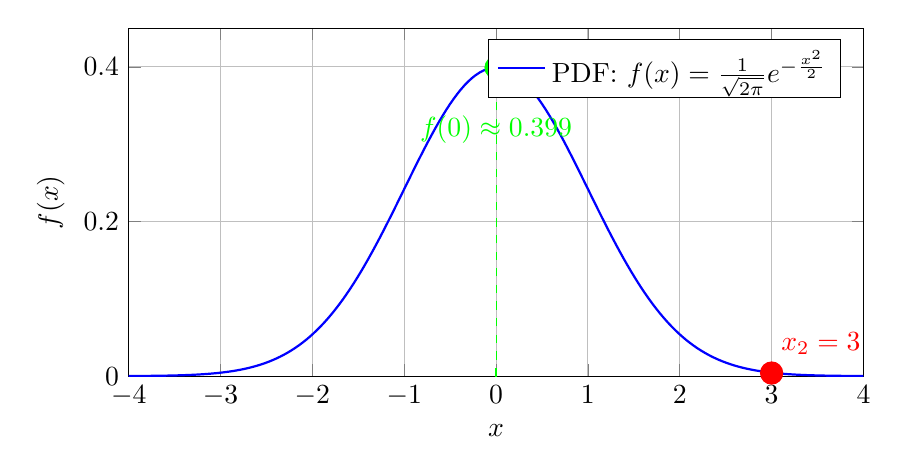
\begin{tikzpicture}
        \begin{axis}[
            width=0.9\textwidth,
            height=6cm,
            xlabel={$x$},
            ylabel={$f(x)$},
            xmin=-4, xmax=4,
            ymin=0, ymax=0.45,
            grid=major,
            legend pos=north east,
            samples=200
        ]
            % Plot the normal distribution PDF
            \addplot[thick, blue, domain=-4:4] {1/sqrt(2*pi) * exp(-x^2/2)};
            \addlegendentry{PDF: $f(x) = \frac{1}{\sqrt{2\pi}} e^{-\frac{x^2}{2}}$}
            
            % Mark x1 = 0 (normal sample)
            \addplot[mark=*, mark size=4pt, color=green, only marks] coordinates {(0, 0.399)};
            \node[above, color=green] at (axis cs: 0, 0.45) {$x_1 = 0$};
            \node[below, color=green] at (axis cs: 0, 0.35) {$f(0) \approx 0.399$};
            \draw[dashed, green] (axis cs: 0, 0) -- (axis cs: 0, 0.399);
            
            % Mark x2 = 3 (outlier)
            \addplot[mark=*, mark size=4pt, color=red, only marks] coordinates {(3, 0.004)};
            \node[above right, color=red] at (axis cs: 3, 0.015) {$x_2 = 3$};
            \node[below, color=red] at (axis cs: 3, -0.02) {$f(3) \approx 0.004$};
            \draw[dashed, red] (axis cs: 3, 0) -- (axis cs: 3, 0.004);
            
            % Add vertical lines to x-axis
            \draw[green, thick] (axis cs: 0, -0.01) -- (axis cs: 0, 0.01);
            \draw[red, thick] (axis cs: 3, -0.01) -- (axis cs: 3, 0.01);
        \end{axis}
    \end{tikzpicture}
    \caption{Probability density function of a standard normal distribution ($\mu = 0$, $\sigma = 1$). The green point at $x_1 = 0$ shows a normal sample with high probability density ($f(0) \approx 0.399$), while the red point at $x_2 = 3$ shows an outlier with very low probability density ($f(3) \approx 0.004$).}
    \label{fig:pdf_anomaly}
\end{figure}

\textbf{Step 1:} Evaluate the probability density for a normal sample $x_1 = 0$ (at the mean):
\begin{equation}
f(0) = \frac{1}{\sqrt{2\pi}} e^{0} \approx 0.399
\end{equation}

\textbf{Step 2:} Calculate the anomaly degree for $x_1$:
\begin{equation}
\text{Anomaly degree} = \frac{1}{f(0)} \approx \frac{1}{0.399} \approx 2.5 \quad \text{(low anomaly)}
\end{equation}

The anomaly degree of 2.5 is considered "low" because it corresponds to a value at the mean of the distribution (most likely value). In practice, anomaly degrees are evaluated \textbf{relative to other samples} in the dataset or compared to a threshold. Common thresholds are based on:
\begin{itemize}
    \item \textbf{Standard deviations}: Values beyond 2-3 standard deviations from the mean
    \item \textbf{Percentiles}: Values below the 1st percentile or above the 99th percentile
    \item \textbf{Relative comparison}: Comparing anomaly degrees across all samples and identifying those significantly higher than the median
\end{itemize}

\textbf{Step 3:} Evaluate the probability density for a potential outlier $x_2 = 3$ (three standard deviations away):
\begin{equation}
f(3) = \frac{1}{\sqrt{2\pi}} e^{-\frac{9}{2}} \approx 0.004
\end{equation}

\textbf{Step 4:} Calculate the anomaly degree for $x_2$:
\begin{equation}
\text{Anomaly degree} = \frac{1}{f(3)} \approx \frac{1}{0.004} \approx 250 \quad \text{(high anomaly)}
\end{equation}

\textbf{Step 5:} Since $x_2$ has a very high anomaly degree (250 vs 2.5), it is identified as an outlier. The comparison shows that $x_2$ has an anomaly degree \textbf{100 times higher} than $x_1$ ($250/2.5 = 100$), indicating it is extremely unlikely and anomalous. In practice, a threshold would be established (e.g., anomaly degree $> 50$ or $> 100$) to automatically flag outliers. Treatment options include: (1) eliminating the value, or (2) replacing it with the mean of its neighboring points.

\subsubsection{Threshold-Based Outlier Detection}

An alternative statistical strategy identifies outliers as values located at the extremes of the domain of a function $f(x)$. This approach defines two threshold values $x_a$ and $x_b$ such that:
\begin{equation}
P(x \leq x_a) = P(x \geq x_b) = P_{\text{min}}
\label{eq:threshold}
\end{equation}
where $P_{\text{min}}$ is a predefined minimum probability threshold. A sample $x_1$ is considered an anomaly if $x_1 < x_a$ or $x_1 > x_b$.

\textbf{Global Application (Point Anomalies):} When applied globally, the function $f(x)$ represents the entire set of available samples (e.g., all points in a time series or all pixels in an image). This approach detects \textbf{point anomalies}, where an individual sample is notably different from the overall dataset.

\textbf{Local Application (Contextual Anomalies):} To identify \textbf{contextual anomalies}, the method is applied within a local environment or neighborhood of the point being studied. Here, $f(x)$ is defined solely based on the neighborhood of the point being evaluated. This involves using a \textbf{sliding window} centered on the target point, similar to how a median filter operates, to define the local context and establish local thresholds $x_a$ and $x_b$ for that specific neighborhood.

\subsubsection{Practical Considerations}

Additionally, both methods based on $f(x)$ require initially setting a \textbf{decision threshold}: 
\begin{itemize}
    \item For the inverse density method: to compare the obtained anomaly score against a threshold
    \item For the threshold-based method: to define the $P_{\text{min}}$ value that identifies the extreme values of a distribution
\end{itemize}

\begin{tcolorbox}[colback=blue!5!white, colframe=blue!75!black, title=\textbf{Important: User-Defined Threshold}]
This threshold determines the definition of anomaly in our dataset and must be established by the user. The choice of threshold directly affects which samples are classified as anomalies, making it a critical parameter in the detection process.
\end{tcolorbox}

In the definition of methods based on the use of the probability density function $f(x)$, knowledge of this function has been assumed. However, in practice, this function is typically \textbf{unknown}, so it is necessary to apply \textbf{estimation techniques} to obtain an approximation of it. The following are some techniques that can be used for estimating this function.

\subsubsection{Estimation Techniques}

\paragraph{Histogram}

This represents the simplest technique. From the samples of a variable, it is discretized by dividing its domain into a limited number of intervals of equal size, identified by their midpoint. These points represent the discrete values that the variable can take. Thus, the frequency (probability) associated with each possible value is obtained from the total initial dataset by counting the number of samples of the variable that fall into each interval.

The choice of the number of intervals used for discretizing the variable has a very significant influence on the obtained approximation. A number that is too small will result in an excessively simple approximation that does not capture the particularities of the target distribution. However, an excessive number of intervals leads to the resulting estimation presenting discontinuities (null values) and abrupt changes in its profile.

\textbf{Example:} Consider a dataset with 20 samples: $\{1.2, 1.5, 1.8, 2.1, 2.3, 2.4, 2.6, 2.7, 2.9, 3.0, 3.1, 3.2, 3.4, 3.5, 3.7, 3.9, 4.2, 4.5, 4.8, 5.1\}$.

\textbf{Step 1:} Divide the domain into intervals. For example, using 5 intervals of width 1.0:
\begin{itemize}
    \item Interval 1: $[1.0, 2.0)$ with midpoint $1.5$
    \item Interval 2: $[2.0, 3.0)$ with midpoint $2.5$
    \item Interval 3: $[3.0, 4.0)$ with midpoint $3.5$
    \item Interval 4: $[4.0, 5.0)$ with midpoint $4.5$
    \item Interval 5: $[5.0, 6.0)$ with midpoint $5.5$
\end{itemize}

\textbf{Step 2:} Count samples in each interval:
\begin{itemize}
    \item Interval 1: 3 samples $\{1.2, 1.5, 1.8\}$ → frequency $= 3/20 = 0.15$
    \item Interval 2: 7 samples $\{2.1, 2.3, 2.4, 2.6, 2.7, 2.9, 3.0\}$ → frequency $= 7/20 = 0.35$
    \item Interval 3: 6 samples $\{3.1, 3.2, 3.4, 3.5, 3.7, 3.9\}$ → frequency $= 6/20 = 0.30$
    \item Interval 4: 3 samples $\{4.2, 4.5, 4.8\}$ → frequency $= 3/20 = 0.15$
    \item Interval 5: 1 sample $\{5.1\}$ → frequency $= 1/20 = 0.05$
\end{itemize}

\textbf{Step 3:} The estimated probability density function assigns to each midpoint the frequency of its interval. For example, $f(2.5) \approx 0.35$ and $f(5.5) \approx 0.05$. A new sample $x = 5.3$ would fall in interval 5, which has low frequency (0.05), indicating it is likely an anomaly.

Figure~\ref{fig:histogram_estimation} visualizes the histogram estimation, showing the frequency bars for each interval. The low frequency in interval 5 (highlighted in red) indicates that values in this range are anomalous.

\begin{figure}[H]
    \centering
    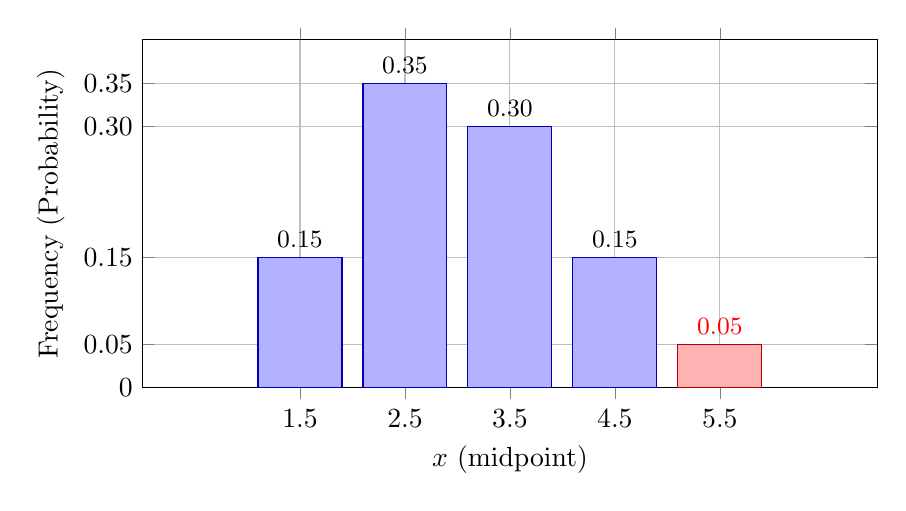
\begin{tikzpicture}
        \begin{axis}[
            width=0.9\textwidth,
            height=6cm,
            xlabel={$x$ (midpoint)},
            ylabel={Frequency (Probability)},
            xmin=1, xmax=6,
            ymin=0, ymax=0.4,
            xtick={1.5, 2.5, 3.5, 4.5, 5.5},
            xticklabels={1.5, 2.5, 3.5, 4.5, 5.5},
            ytick={0, 0.05, 0.15, 0.30, 0.35},
            yticklabels={0, 0.05, 0.15, 0.30, 0.35},
            grid=major,
            bar width=0.8,
            ybar,
            bar shift=0pt,
            enlarge x limits=0.2
        ]
            % Histogram bars
            \addplot[fill=blue!30, draw=blue!70!black] coordinates {
                (1.5, 0.15)
                (2.5, 0.35)
                (3.5, 0.30)
                (4.5, 0.15)
            };
            
            % Anomalous interval (low frequency)
            \addplot[fill=red!30, draw=red!70!black] coordinates {
                (5.5, 0.05)
            };
            
            % Add labels on bars
            \node[above] at (axis cs: 1.5, 0.15) {\small 0.15};
            \node[above] at (axis cs: 2.5, 0.35) {\small 0.35};
            \node[above] at (axis cs: 3.5, 0.30) {\small 0.30};
            \node[above] at (axis cs: 4.5, 0.15) {\small 0.15};
            \node[above, color=red] at (axis cs: 5.5, 0.05) {\small 0.05};
            
            % Mark anomaly region
            \node[below, color=red] at (axis cs: 5.5, -0.02) {\small Anomaly};
        \end{axis}
    \end{tikzpicture}
    \caption{Histogram estimation of probability density function. Each bar represents the frequency (probability) of samples in that interval. The red bar (interval 5) has very low frequency (0.05), indicating anomalous values.}
    \label{fig:histogram_estimation}
\end{figure}

\textbf{Note:} If we had used only 2 intervals, we would lose detail about the distribution shape. If we used 20 intervals (one per sample), many intervals would have zero frequency, creating discontinuities.

\paragraph{Kernel Density Estimation}

Kernel Density Estimation (KDE) is a non-parametric method that provides a smooth estimate of the probability density function. Instead of using fixed intervals like histograms, KDE places a "kernel" (a smooth function, typically a Gaussian) centered at each data point and sums these kernels to create a continuous density estimate.

The estimated density function is given by:
\begin{equation}
\hat{f}(x) = \frac{1}{nh} \sum_{i=1}^{n} K\left(\frac{x - x_i}{h}\right)
\label{eq:kde}
\end{equation}
where $n$ is the number of samples, $h$ is the bandwidth (smoothing parameter), $x_i$ are the data points, and $K$ is the kernel function. A common choice is the Gaussian kernel: $K(u) = \frac{1}{\sqrt{2\pi}} e^{-\frac{u^2}{2}}$.

\begin{tcolorbox}[colback=blue!5!white, colframe=blue!75!black, title=\textbf{Curious Fact: What is a Kernel?}]
A \textbf{kernel} is a smooth, symmetric function that assigns weights to nearby data points. Think of it as a "bump" or "hill" centered at each data point that spreads influence to nearby regions.

Key properties of kernels:
\begin{itemize}
    \item \textbf{Symmetric}: $K(-u) = K(u)$ for all $u$
    \item \textbf{Non-negative}: $K(u) \geq 0$ for all $u$
    \item \textbf{Integrates to 1}: $\int_{-\infty}^{\infty} K(u) \, du = 1$ (ensures the density estimate is valid)
    \item \textbf{Peak at center}: Maximum value occurs at $u = 0$
\end{itemize}

The Gaussian kernel is most common because it's smooth and has infinite support, meaning it gives non-zero weight to all points (though very small for distant points). Other kernel types include uniform, triangular, and Epanechnikov kernels. The kernel essentially "smears" each data point's influence across its neighborhood, creating a smooth density estimate when all kernels are summed together.
\end{tcolorbox}

The bandwidth $h$ plays a crucial role: a small $h$ creates a detailed but noisy estimate, while a large $h$ produces a smoother but potentially oversimplified estimate.

\textbf{Example:} Using the same dataset as before: $\{1.2, 1.5, 1.8, 2.1, 2.3, 2.4, 2.6, 2.7, 2.9, 3.0, 3.1, 3.2, 3.4, 3.5, 3.7, 3.9, 4.2, 4.5, 4.8, 5.1\}$.

\textbf{Step 1:} Choose a bandwidth. For this example, let $h = 0.5$ (moderate smoothing).

\textbf{Step 2:} For any point $x$, calculate the density estimate by summing Gaussian kernels centered at each data point. For example, at $x = 2.5$:
\begin{equation}
\hat{f}(2.5) = \frac{1}{20 \times 0.5} \sum_{i=1}^{20} \frac{1}{\sqrt{2\pi}} e^{-\frac{(2.5 - x_i)^2}{2 \times 0.5^2}}
\end{equation}
This gives a smooth, continuous estimate of the density.

\textbf{Step 3:} For an anomalous point $x = 5.3$, the density estimate will be very low because it is far from most data points. The kernels centered at nearby points (like $x_i = 5.1$) contribute little, and kernels from distant points contribute almost nothing, resulting in $\hat{f}(5.3) \approx 0.02$, indicating an anomaly.

Figure~\ref{fig:kde_estimation} compares the histogram and KDE estimates, showing how KDE provides a smooth continuous curve without discontinuities.

\begin{figure}[H]
    \centering
    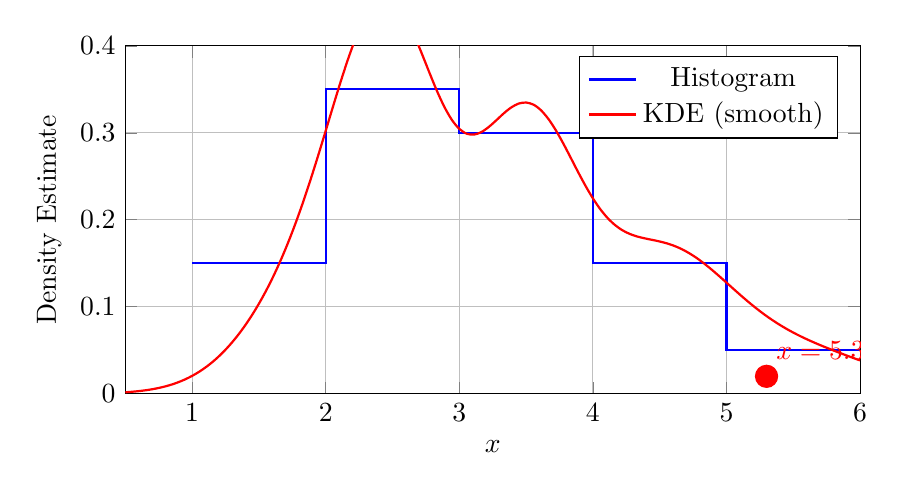
\begin{tikzpicture}
        \begin{axis}[
            width=0.9\textwidth,
            height=6cm,
            xlabel={$x$},
            ylabel={Density Estimate},
            xmin=0.5, xmax=6,
            ymin=0, ymax=0.4,
            grid=major,
            legend pos=north east
        ]
            % Histogram (step function approximation)
            \addplot[thick, blue, const plot, samples=5] coordinates {
                (1, 0.15) (2, 0.15)
                (2, 0.35) (3, 0.35)
                (3, 0.30) (4, 0.30)
                (4, 0.15) (5, 0.15)
                (5, 0.05) (6, 0.05)
            };
            \addlegendentry{Histogram}
            
            % KDE smooth curve (approximation)
            \addplot[thick, red, smooth, samples=100, domain=0.5:6] {
                0.15*exp(-((x-2)^2)/0.5) + 
                0.35*exp(-((x-2.5)^2)/0.3) + 
                0.30*exp(-((x-3.5)^2)/0.3) + 
                0.15*exp(-((x-4.5)^2)/0.5) + 
                0.05*exp(-((x-5.5)^2)/0.8)
            };
            \addlegendentry{KDE (smooth)}
            
            % Mark anomaly region
            \addplot[mark=*, mark size=4pt, color=red, only marks] coordinates {(5.3, 0.02)};
            \node[above right, color=red] at (axis cs: 5.3, 0.02) {$x=5.3$ (anomaly)};
        \end{axis}
    \end{tikzpicture}
    \caption{Comparison of histogram and kernel density estimation. The histogram (blue) shows discrete intervals, while KDE (red) provides a smooth continuous estimate. The point $x=5.3$ has very low density in both methods, indicating an anomaly.}
    \label{fig:kde_estimation}
\end{figure}

\paragraph{Parametric Estimation}

It is assumed that the probability density function that statistically characterizes the variable is of normal type. Therefore, the mean and variance of this distribution are the parameters to be obtained. For this, the estimations derived from the available sample are used:

\begin{tcolorbox}[colback=blue!5!white, colframe=blue!75!black, title=\textbf{Curious Fact: What is "Normal Type"?}]
A \textbf{normal distribution} (also called Gaussian distribution) is a bell-shaped, symmetric probability distribution that is one of the most important distributions in statistics. It is called "normal" because many natural phenomena approximately follow this distribution.

Key characteristics:
\begin{itemize}
    \item \textbf{Bell-shaped curve}: Symmetric around the mean, with a single peak
    \item \textbf{Completely determined by two parameters}: Mean $\mu$ (center) and variance $\sigma^2$ (spread)
    \item \textbf{68-95-99.7 rule}: Approximately 68\% of data falls within 1 standard deviation, 95\% within 2, and 99.7\% within 3 standard deviations of the mean
    \item \textbf{Common in nature}: Many measurements (heights, test scores, measurement errors) tend to follow normal distributions due to the Central Limit Theorem
\end{itemize}

When we say a variable is "of normal type," we mean its probability density function follows the normal distribution formula. This assumption simplifies estimation because we only need to estimate two parameters ($\mu$ and $\sigma^2$) instead of the entire function shape.
\end{tcolorbox}

\begin{equation}
\mu_x = \frac{1}{n} \sum_{i=1}^{n} x_i
\label{eq:mean_est}
\end{equation}

\begin{equation}
\sigma_x^2 = \frac{1}{n} \sum_{i=1}^{n} (x_i - \mu_x)^2
\label{eq:variance_est}
\end{equation}

\textbf{Breaking down the equations:}

\textbf{Equation~\ref{eq:mean_est} (Sample Mean):}
\begin{itemize}
    \item $\mu_x$: The estimated mean (average) of the data
    \item $n$: Total number of samples in the dataset
    \item $\sum_{i=1}^{n}$: Summation symbol, meaning "add up all values from $i=1$ to $i=n$"
    \item $x_i$: The $i$-th individual observation/value in the dataset
    \item $\frac{1}{n}$: Dividing by $n$ to get the average (mean)
\end{itemize}
\textit{In simple terms:} Add up all the values and divide by the number of values to get the average.

\textbf{Equation~\ref{eq:variance_est} (Sample Variance):}
\begin{itemize}
    \item $\sigma_x^2$: The estimated variance (measure of spread/dispersion)
    \item $n$: Total number of samples
    \item $(x_i - \mu_x)$: The difference between each value and the mean (how far each point is from the center)
    \item $(x_i - \mu_x)^2$: Squaring the difference (ensures all values are positive and emphasizes larger deviations)
    \item $\sum_{i=1}^{n}$: Sum all the squared differences
    \item $\frac{1}{n}$: Average of the squared differences
\end{itemize}
\textit{In simple terms:} Calculate how far each value is from the mean, square those distances, then average them. This measures how spread out the data is around the mean.

Once these parameters are estimated, the normal probability density function can be fully specified as:

\begin{equation}
f(x) = \frac{1}{\sigma_x\sqrt{2\pi}} e^{-\frac{(x-\mu_x)^2}{2\sigma_x^2}}
\end{equation}

This parametric approach is simpler than non-parametric methods but requires the assumption that the data follows a normal distribution, which may not always be valid.

Obviously, the main limitation of this method comes from the initial assumption about the shape of the distribution. The error in the estimation will be more significant, therefore, the more the real distribution of the variable differs from the normal profile initially assumed. If the data is highly skewed, multimodal, or has heavy tails, the normal assumption will lead to poor density estimates and consequently, inaccurate anomaly detection.

\paragraph{Kernel Functions (Parzen Method)}

This is a hybrid procedure between histogram-based estimation and parametric estimation. In this case, the estimation of the probability density function is given by the superposition of kernel functions centered at each of the initially observed samples $x_i$. The expression for the estimated function is obtained as follows:

\begin{equation}
\hat{f}(x) = \frac{1}{n} \sum_{i=1}^{n} g(x - x_i, \theta)
\label{eq:parzen}
\end{equation}

where:
\begin{itemize}
    \item $g(x, \theta)$ is the kernel function
    \item $\theta$ represents the set of parameters for this function (e.g., bandwidth $h$ in the Gaussian kernel case)
\end{itemize}

This formulation is equivalent to the Kernel Density Estimation (KDE) method described earlier, where the kernel function $g(x - x_i, \theta)$ corresponds to $K((x-x_i)/h)$ scaled appropriately. The Parzen window method provides a unified framework that bridges discrete histogram methods and continuous parametric approaches.

\textbf{Example:} Using the same dataset: $\{1.2, 1.5, 1.8, 2.1, 2.3, 2.4, 2.6, 2.7, 2.9, 3.0, 3.1, 3.2, 3.4, 3.5, 3.7, 3.9, 4.2, 4.5, 4.8, 5.1\}$ with $n = 20$ samples.

\textbf{Step 1:} Choose a kernel function and its parameters. For this example, we use a Gaussian kernel with bandwidth $h = 0.5$:
\begin{equation}
g(x - x_i, \theta) = g(x - x_i, h) = \frac{1}{h\sqrt{2\pi}} e^{-\frac{(x - x_i)^2}{2h^2}}
\end{equation}

\textbf{Step 2:} To estimate the density at any point $x$, sum the kernel functions centered at each data point. For example, at $x = 2.5$:
\begin{equation}
\hat{f}(2.5) = \frac{1}{20} \sum_{i=1}^{20} \frac{1}{0.5\sqrt{2\pi}} e^{-\frac{(2.5 - x_i)^2}{2 \times 0.5^2}}
\end{equation}
Each term in the sum represents the contribution of one data point $x_i$ to the density estimate at $x = 2.5$. Points closer to 2.5 contribute more (higher kernel value), while distant points contribute less.

\textbf{Step 3:} For an anomalous point $x = 5.3$, most kernel functions centered at the data points will have very small values because $5.3$ is far from most samples. The only significant contribution comes from the kernel centered at $x_i = 5.1$, resulting in $\hat{f}(5.3) \approx 0.02$, indicating an anomaly.

\textbf{Visualization:} The Parzen window method creates a smooth density estimate by placing a "bump" (kernel) at each data point and summing all bumps. The height of the resulting curve at any point $x$ represents the estimated probability density, with low values indicating potential anomalies.

Figure~\ref{fig:parzen_visualization} illustrates the Parzen window method, showing individual kernel functions (Gaussian bumps) centered at sample data points and the resulting density estimate obtained by summing all kernels.

\begin{figure}[H]
    \centering
    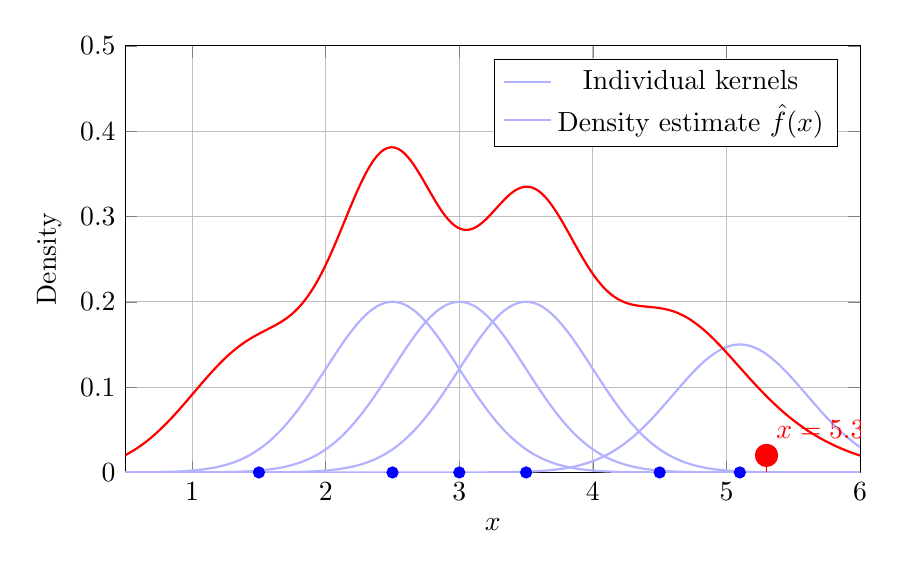
\begin{tikzpicture}
        \begin{axis}[
            width=0.9\textwidth,
            height=7cm,
            xlabel={$x$},
            ylabel={Density},
            xmin=0.5, xmax=6,
            ymin=0, ymax=0.5,
            grid=major,
            legend pos=north east
        ]
            % Sample data points (some representative ones)
            \def\samples{1.5, 2.5, 3.0, 3.5, 4.5, 5.1}
            
            % Draw individual kernels (bumps) at some data points
            \addplot[thick, blue!30, smooth, samples=100, domain=0.5:6] {
                0.2*exp(-((x-2.5)^2)/0.5)
            };
            \addlegendentry{Individual kernels}
            
            \addplot[thick, blue!30, smooth, samples=100, domain=0.5:6] {
                0.2*exp(-((x-3.0)^2)/0.5)
            };
            
            \addplot[thick, blue!30, smooth, samples=100, domain=0.5:6] {
                0.2*exp(-((x-3.5)^2)/0.5)
            };
            
            \addplot[thick, blue!30, smooth, samples=100, domain=0.5:6] {
                0.15*exp(-((x-5.1)^2)/0.5)
            };
            
            % Resulting density estimate (sum of all kernels - approximation)
            \addplot[thick, red, smooth, samples=200, domain=0.5:6] {
                0.15*exp(-((x-1.5)^2)/0.5) + 
                0.35*exp(-((x-2.5)^2)/0.3) + 
                0.30*exp(-((x-3.5)^2)/0.3) + 
                0.15*exp(-((x-4.5)^2)/0.5) + 
                0.05*exp(-((x-5.1)^2)/0.8)
            };
            \addlegendentry{Density estimate $\hat{f}(x)$}
            
            % Mark data points
            \addplot[mark=*, mark size=2pt, color=blue, only marks] coordinates {
                (1.5, 0) (2.5, 0) (3.0, 0) (3.5, 0) (4.5, 0) (5.1, 0)
            };
            
            % Mark anomaly point
            \addplot[mark=*, mark size=4pt, color=red, only marks] coordinates {(5.3, 0.02)};
            \node[above right, color=red] at (axis cs: 5.3, 0.02) {$x=5.3$ (anomaly)};
            
            % Draw vertical line at anomaly
            \draw[dashed, red] (axis cs: 5.3, 0) -- (axis cs: 5.3, 0.02);
        \end{axis}
    \end{tikzpicture}
    \caption{Parzen window method visualization. Individual Gaussian kernels (blue, semi-transparent) are centered at each data point. The resulting density estimate (red curve) is obtained by summing all kernels. The point $x=5.3$ has very low density, indicating an anomaly.}
    \label{fig:parzen_visualization}
\end{figure}

Commonly, a Gaussian normal is used as the kernel function, so that the parameter set $\theta$ is given solely by the variance of the normal, since each kernel function is centered at the corresponding sample. It is common to use the same variance value for all kernel functions, so the estimated probability density function would be obtained as:

\begin{equation}
\hat{f}(x) = \frac{1}{n} \sum_{i=1}^{n} \frac{1}{\sqrt{2\pi\sigma^2}} \exp\left[-\frac{(x-x_i)^2}{2\sigma^2}\right]
\label{eq:gaussian_parzen}
\end{equation}

where $\sigma^2$ is the variance parameter (bandwidth) that controls the width of each Gaussian kernel. As observed, the effect of the variance of the normal kernel functions is similar to the interval size for histogram calculation. In fact, the histogram can be seen as a particular case of kernel-based estimation, in which these functions would be given by uniform pulses of unit height centered at the midpoint of each interval.

\begin{tcolorbox}[colback=blue!5!white, colframe=blue!75!black, title=\textbf{Understanding the Relationship: Histogram vs. Kernel Estimation}]
\textbf{Similarity:} Both histogram interval size and kernel variance control the \textbf{smoothing} of the density estimate:
\begin{itemize}
    \item \textbf{Large histogram intervals} or \textbf{large kernel variance} $\sigma^2$: Produce smoother, less detailed estimates (may oversimplify)
    \item \textbf{Small histogram intervals} or \textbf{small kernel variance} $\sigma^2$: Produce more detailed, potentially noisy estimates (may overfit)
\end{itemize}

\textbf{Histogram as a special case:} A histogram can be viewed as kernel estimation using:
\begin{itemize}
    \item \textbf{Uniform kernels} (rectangular pulses) instead of smooth Gaussian kernels
    \item Kernels of \textbf{unit height} and \textbf{width equal to the interval size}
    \item Kernels \textbf{centered at interval midpoints} rather than at individual data points
\end{itemize}

The key difference is that histograms use \textbf{discrete, non-overlapping} uniform kernels, while kernel density estimation uses \textbf{continuous, overlapping} smooth kernels (typically Gaussian), resulting in a smoother density estimate.
\end{tcolorbox}

A common rule for obtaining an adequate value of the variance of kernel functions is to set it to the following value:

\begin{equation}
\sigma = 1.06 \sigma_x n^{-1/5}
\label{eq:silverman_rule}
\end{equation}

where $\sigma_x$ is the standard deviation of the sample data and $n$ is the number of samples. This is known as \textbf{Silverman's rule of thumb} for bandwidth selection. The factor $1.06$ is optimal for Gaussian kernels when the underlying distribution is approximately normal, and the term $n^{-1/5}$ ensures that the bandwidth decreases as the sample size increases, allowing for more detailed estimates with more data.

This rule provides a good starting point for kernel variance selection, balancing between oversmoothing (too large $\sigma$) and undersmoothing (too small $\sigma$).

